%---------------------------------------------------------------------
%
%                  Project Name: Radar System Network Report
%
%---------------------------------------------------------------------
%
%                 created by LuoMin <luomin5417@gmail.com>
%
%                        Last-modified: 2018-5-18
%
%---------------------------------------------------------------------

\documentclass[a4paper,12pt]{report}
\usepackage{etex}
\usepackage{ctex}
%\usepackage{xeCJK}
\usepackage{times}
\usepackage{setspace}
\usepackage{fancyhdr}
\usepackage{graphicx}
\usepackage{wrapfig}
\usepackage{array}  
\usepackage{fontspec,xunicode,xltxtra}
\usepackage{titlesec}
\usepackage{titletoc}
\usepackage[titletoc]{appendix}
\usepackage[top=30mm,bottom=30mm,left=20mm,right=20mm]{geometry}
\usepackage{cite}
\usepackage{listings}
\usepackage{caption,subcaption}
\usepackage[framed,numbered,autolinebreaks,useliterate]{mcode} % 插入代码
\usepackage{xeboiboites}
\usepackage{amsmath,amssymb}
\usepackage{hyperref}
\usepackage{float}

\usepackage{xcolor}
\usepackage{tcolorbox}

\RequirePackage{tkz-network}

\hypersetup{hidelinks}

\XeTeXlinebreaklocale "zh"
\XeTeXlinebreakskip = 0pt plus 1pt minus 0.1pt

%---------------------------------------------------------------------
%	页眉页脚设置
%---------------------------------------------------------------------
\fancypagestyle{plain}{
	\pagestyle{fancy}      %改变章节首页页眉
}

\pagestyle{fancy}
\lhead{\kaishu~宜通华盛~}
\rhead{\kaishu~研发部~}
\cfoot{\thepage}

%---------------------------------------------------------------------
%	章节标题设置
%---------------------------------------------------------------------
\titleformat{\chapter}{\centering\zihao{-1}\heiti}{第\chinese{chapter}章}{1em}{}
\titlespacing{\chapter}{0pt}{*0}{*6}

%---------------------------------------------------------------------
%	摘要标题设置
%---------------------------------------------------------------------
\renewcommand{\abstractname}{\zihao{-3} 摘\quad 要}

%---------------------------------------------------------------------
%	参考文献设置
%---------------------------------------------------------------------
\renewcommand{\bibname}{\zihao{2}{\hspace{\fill}参\hspace{0.5em}考\hspace{0.5em}文\hspace{0.5em}献\hspace{\fill}}}

%---------------------------------------------------------------------
%	引用文献设置为上标
%---------------------------------------------------------------------
\makeatletter
\def\@cite#1#2{\textsuperscript{[{#1\if@tempswa , #2\fi}]}}
\makeatother

%---------------------------------------------------------------------
%	目录页设置
%---------------------------------------------------------------------
\titlecontents{chapter}[0em]{\songti\zihao{-4}}{\thecontentslabel\ }{}
{\hspace{.5em}\titlerule*[4pt]{$\cdot$}\contentspage}
\titlecontents{section}[2em]{\vspace{0.1\baselineskip}\songti\zihao{-4}}{\thecontentslabel\ }{}
{\hspace{.5em}\titlerule*[4pt]{$\cdot$}\contentspage}
\titlecontents{subsection}[4em]{\vspace{0.1\baselineskip}\songti\zihao{-4}}{\thecontentslabel\ }{}
{\hspace{.5em}\titlerule*[4pt]{$\cdot$}\contentspage}

%---------------------------------------------------------------------
%	公式设置
%---------------------------------------------------------------------
%%define the newthem environment
\newboxedtheorem[small box style={fill=blue!20,draw=black, 
    rounded corners},
    big box style={fill=blue!10,draw=orange,thick,rounded corners},
    headfont=\bfseries]%
    {proposition}{公式}{somecounter} 

%---------------------------------------------------------------------
%   生成大纲
%---------------------------------------------------------------------

\begin{document}
%---------------------------------------------------------------------
%	封面设置
%---------------------------------------------------------------------
\begin{titlepage}
	\begin{center}
		
    
\includegraphics[width=0.9\textwidth]{figure//etws.png}\\
    \vspace{40mm}
    \textbf{\zihao{2}\kaishu{ETWS-1609雷达系统}}\\[0.8cm]
    \textbf{\zihao{2}\kaishu{网络管理设计方案}}\\[3cm]
    
	\vspace{\fill}
	
\setlength{\extrarowheight}{3mm}
{\songti\zihao{3}	
\begin{tabular}{rl}
	
	{\makebox[4\ccwd][s]{部\qquad 门:}}& ~\kaishu 研发部\\
	
	{\makebox[4\ccwd][s]{编\qquad 制:}}& ~\kaishu 罗敏 \\ 

\end{tabular}
 }\\[2cm]
\vspace{\fill}
\zihao{4}
使用\LaTeX 撰写于\today
	\end{center}	
\end{titlepage}

%---------------------------------------------------------------------
%  摘要页
%---------------------------------------------------------------------
\begin{abstract}
\begin{spacing}{1.5}
	{\zihao{-4}
	本文主要是关于雷达系统远程控制网络的管理方案设计,目的是实现全国各地雷达系统的远程监
	测与控制,主要是从两个方面来考虑如何设计实现,第一是从可操作性方面来考虑,因整个控制
	网连接的设备较多,特别是雷达设备甚至可能是位于郊区等人迹罕至的地方,将所有的接入设备
	都连接固定IP专网接口是不太现实的,而且费用过高,方案必须符合实际具有可操作性。第二个
	是从安全性的角度,整个系统分布与全国各地,且连接的雷达用户各不相同,需要考虑用户之间
	的隔离,以及防止非法的网络入侵破坏雷达系统工作。要实现这两个目的,可行的方案是采用
	VPN技术,将分布于各地的雷达设备、控制主机和后端管理服务器配置成为一个虚拟专网,这样
	的设计只需要位于后端的VPN服务器一个固定IP,其它设备只需要连接普通的互联网服务便可以
	实现目的,费用低廉具有可操作性,且VPN的数据传输采用了多重加密技术可以有效防止数据泄
	露。

	\textbf{关键字}:\quad 远程监控 \quad VPN \quad 虚拟专网 \quad 安全性
	}
\end{spacing}
\end{abstract}

%---------------------------------------------------------------------
%  目录页
%---------------------------------------------------------------------
\tableofcontents % 生成目录

%---------------------------------------------------------------------
%  第一章
%---------------------------------------------------------------------
\chapter{设计方案}
\setcounter{page}{1}
\begin{spacing}{1.5}
\songti\zihao{-4}

\section{系统结构}
要对整个雷达系统进行网络设计,则需要先弄楚整个雷达系统的结构组成,下面主要对雷达系统的特
点进行了一些总结:
\begin{itemize}
\itemsep=3pt
\parskip=0pt
\setlength{\itemindent}{1em} 
\item 系统庞大设备多,包括雷达、控制服务器、监控摄像头、UPS设备等等
\item 设备分散位于全国各地,后期可能还会不停的在各个地方扩展
\item 需要时时监控设备工作情况,随时获取雷达数据
\end{itemize}

整个系统的结构如图1.1所示:
\begin{figure}[hbtp]
	\centering
	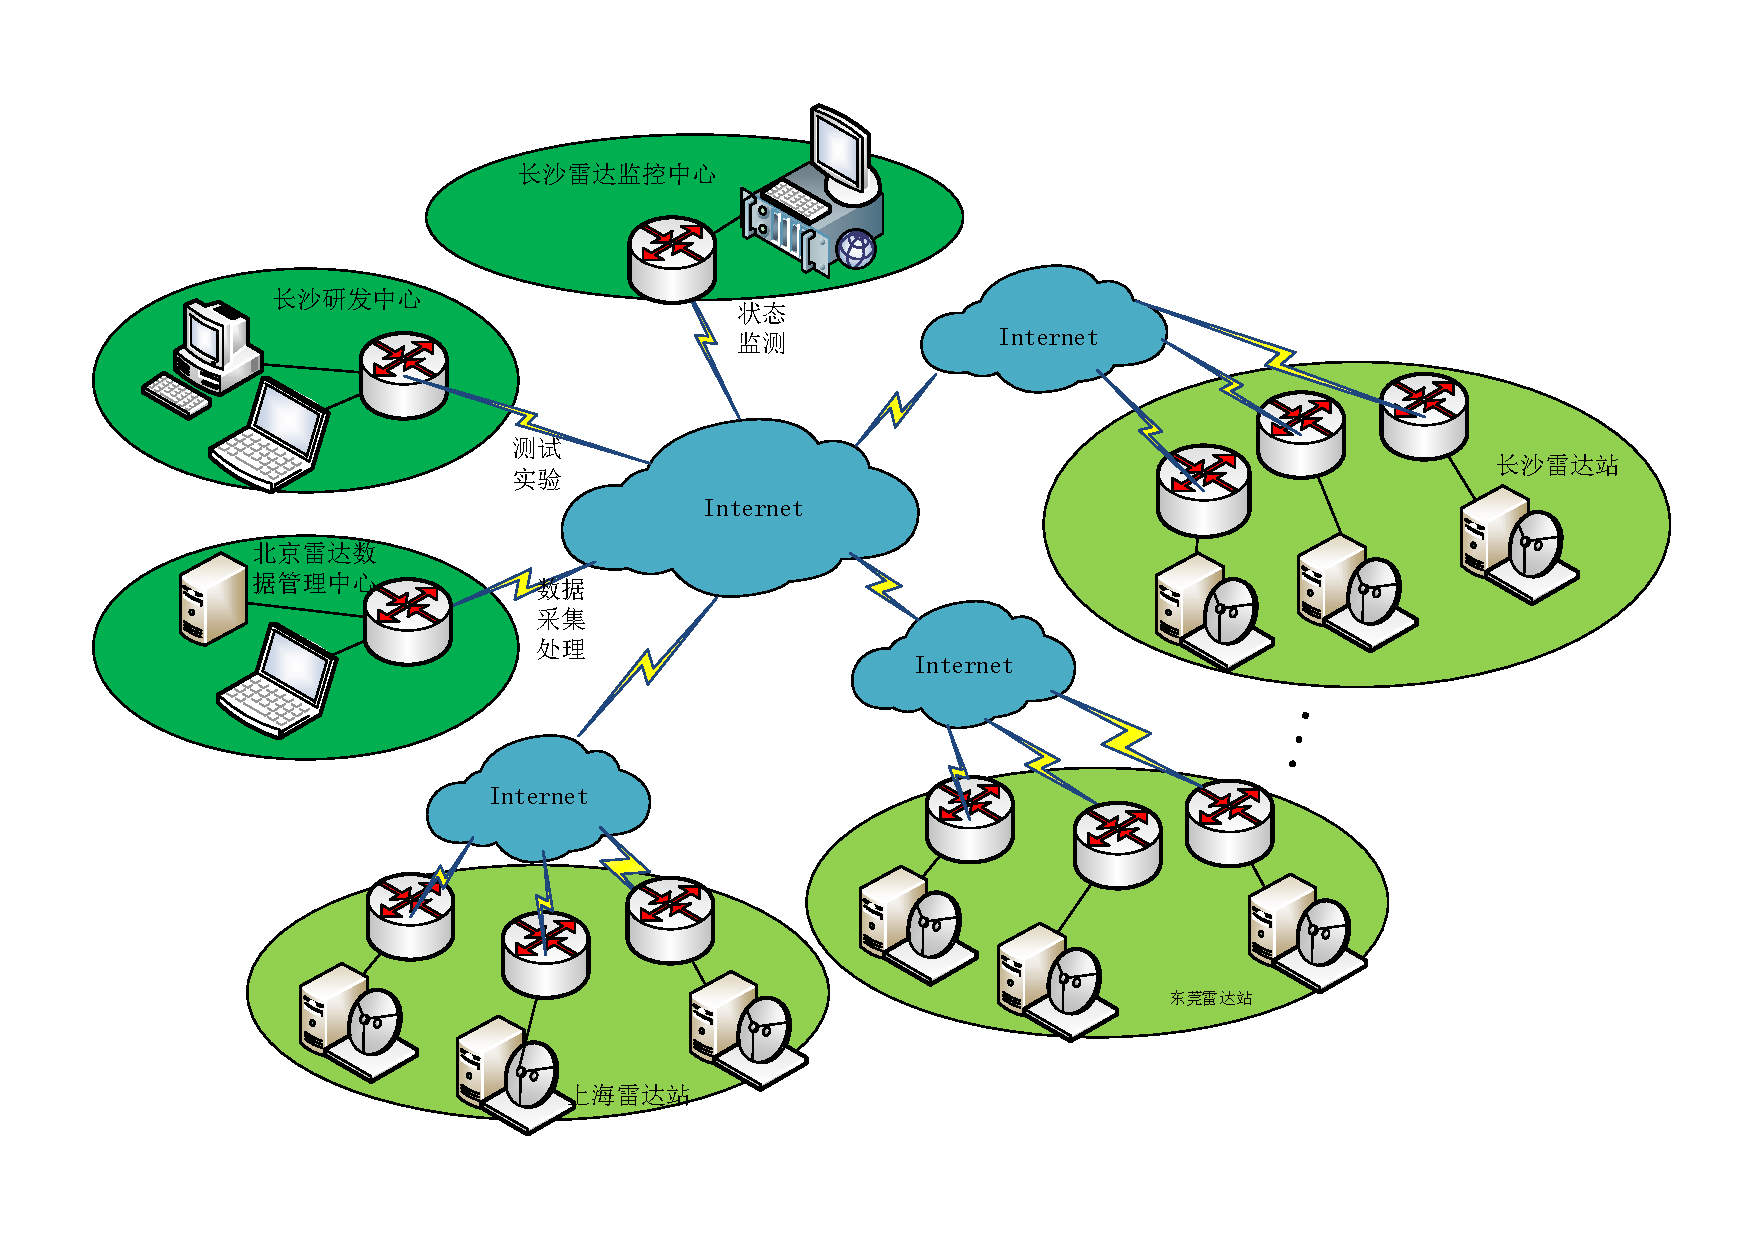
\includegraphics [width=1.0\textwidth]{figure//RadarSystem.pdf}
	\caption{雷达系统结构图}\label{RadarSystem}
\end{figure}

在图1.1可以看到雷达系统组成结构复杂,每个站点有多台雷达,不同站点的雷达也是各自分散的,
根据目前的发展情况,后续还会增加更多的雷达站点,除了雷达站点之外雷达系统的监控管理中心
在长沙,长沙的研发中心也会有访问雷达站点进行实验测试的需求,北京雷达数据管理中心则是主要
需要从各个雷达站点读取数据进行雷达数据的处理。

\section{网络设计}
上一节简单的介绍了整个雷达系统的结构,本节根据雷达系统的结构,进行网络管理方案设计。针对
目前的情况和现有的技术,本文决定采用VPN技术组建私有专网,具体组网方案如图1.2所示:
\begin{figure}[hbtp]
	\centering
	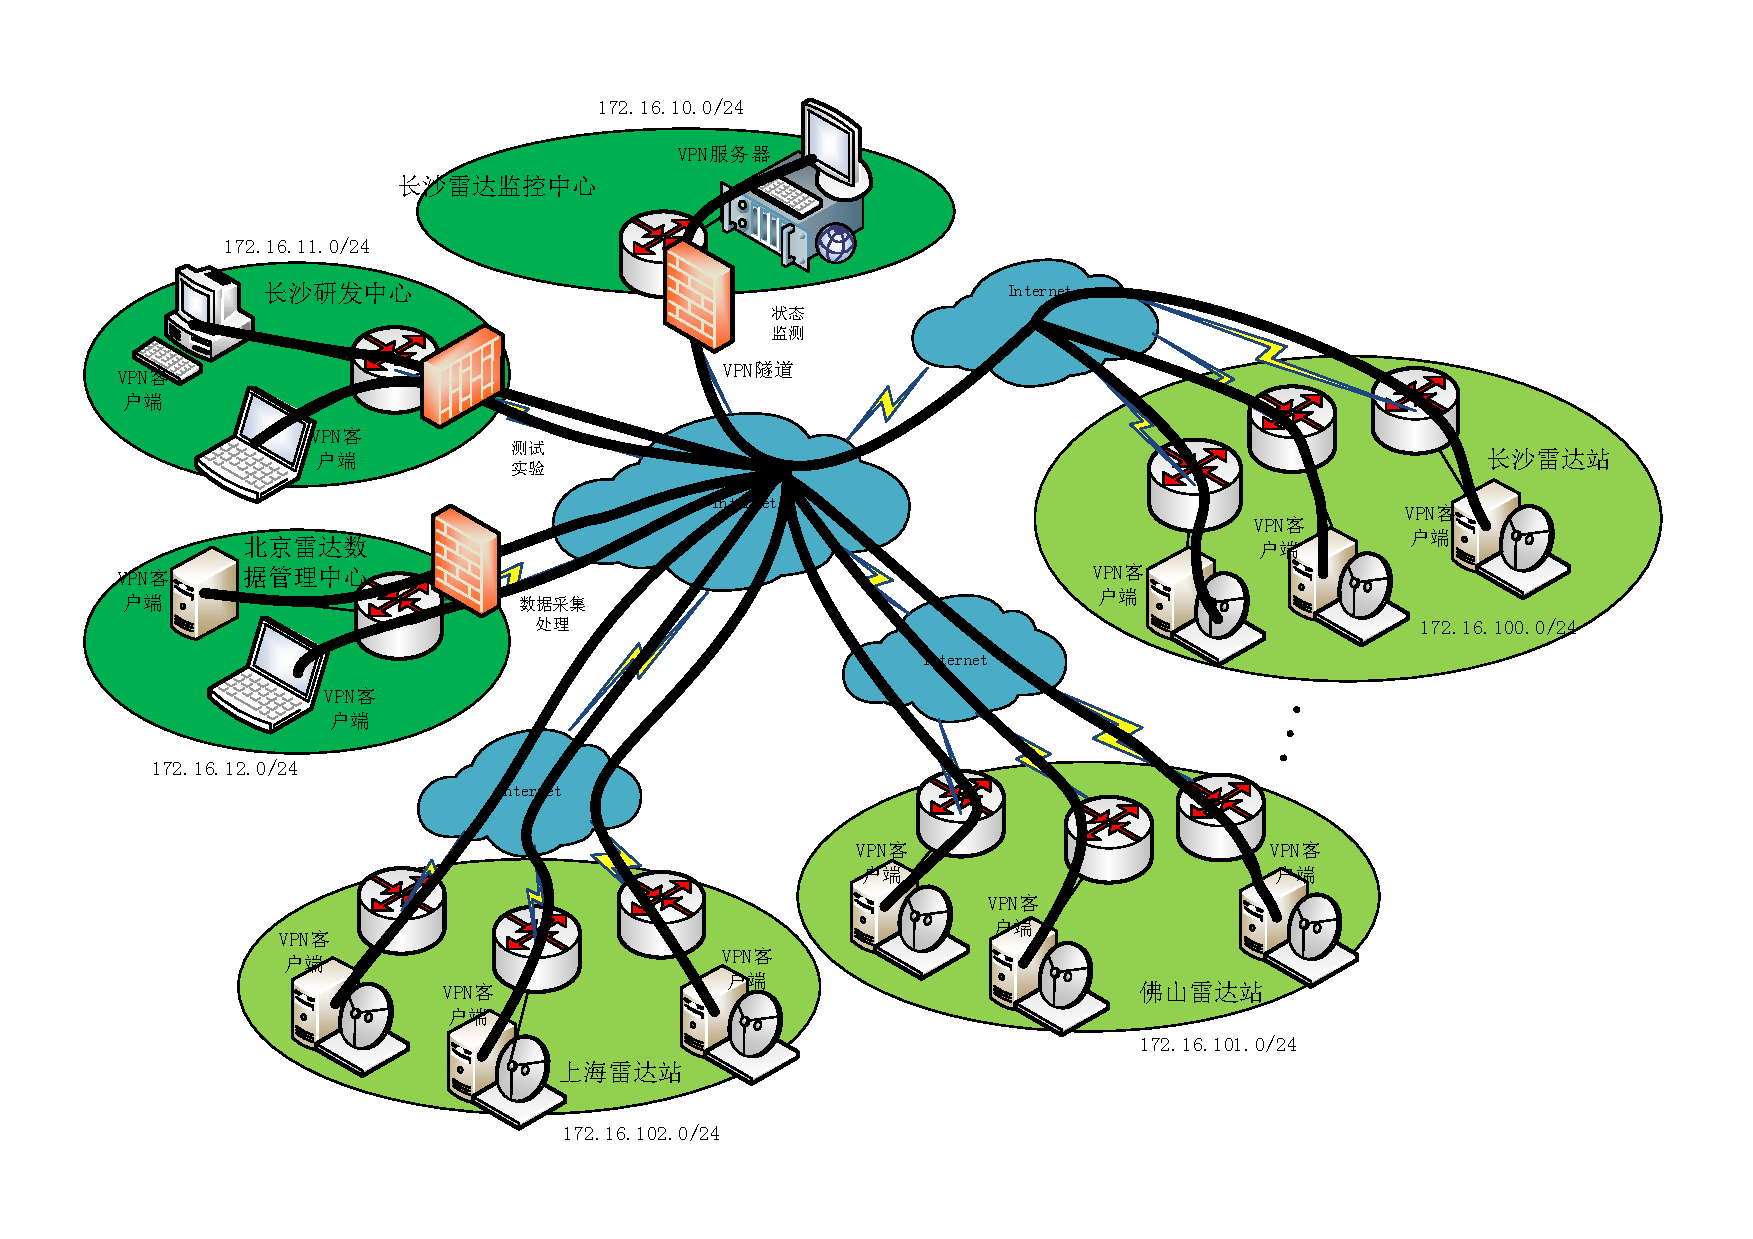
\includegraphics [width=1.0\textwidth]{figure//RadarNet.pdf}
	\caption{雷达系统网络设计}\label{RadarNet}
\end{figure}

在长沙雷达管理中心设置一台VPN服务器,来提供VPN服务管理,其它的网络节点,则通过VPN客户端
远程加入VPN网络,因此长沙雷达管理中心需要一个专网IP,以便其它节点可以方便访问。为了系统
安全还需要进行网络隔离,各个雷达站之间不能相互访问,同时需要在各个管理中心添加防火墙,防
止雷达站访问到网络中心。

目前考虑没有能够满足要求的集成VPN路由器,只能采用在雷达设备的内部服务器上配置VPN客户端,
后期可以考虑我司自主设计一个多功能网关设备作为雷达站点的控制网关,届时可以将VPN客户端
配置在多功能集成网关上。

\section{网络划分}
在图1.2中标注的网络地址是指在接入VPN专网时分配的虚拟局域网IP地址,具体规划网段如表1.1。
\begin{table}[hbtp]
	\centering
	\begin{tabular}{|l|c|c|c|}
	\hline
	区域 & IP地址段 & 特殊地址 & 备注\\
	\hline
	长沙监控中心 & 172.16.10.0/24  & 172.16.10.1   & VPN服务器地址\\
	\hline
	长沙研发中心 & 172.16.11.0/24  & - & -\\
	\hline
	北京数据中心 & 172.16.12.0/24  & 172.16.12.100 & 数据服务器地址\\
	\hline
	长沙雷达站   & 172.16.100.0/24 & 172.16.100.10-172.16.100.12 & 雷达设备地址\\
	\hline
	佛山雷达站   & 172.16.101.0/24 & 172.16.101.10-172.16.101.16 & 雷达设备地址\\
	\hline
	上海雷达站   & 172.16.102.0/24 & 172.16.102.10-172.16.102.12 & 雷达设备地址\\
	\hline
	...    		& ...             & ... & ...\\
	\hline
	\end{tabular}
	\caption{VPN专网IP地址划分}
	\label{tab:IPaddress}
\end{table}

表中目前只列出了部分地区的IP地址网段,后续根据雷达站的部署可以添加地址网段划分,但是基本
的地址划分遵循以下个原则:
\begin{itemize}
\itemsep=3pt
\parskip=0pt
\setlength{\itemindent}{1em} 
\item[-] 整个VPN虚拟专网使用172.16.0.0/16网段
\item[-] 长沙监控中心使用172.16.10.0/24网段,VPN服务器使用172.16.10.1IP地址
\item[-] 长沙研发中心使用172.16.11.0/24网段,接入设备自动分配IP
\item[-] 北京数据中心使用172.16.12.0/24网段,数据服务器使用用172.16.12.100地址,其它
接入设备自动分配IP
\item[-] 雷达站使用172.16.100.0/24-172.16.254.0/24网段,具体根据入网先后编址
\item[-] 雷达设备使用172.16.10x.10-172.16.10x.127的固定地址
\end{itemize}

清晰的编址可以有效的定位设备、判断问题,是雷达系统网络设备管理的基础,后续根据讨论之后可
以根据讨论之后加入新的编址原则以便更好的管理雷达系统网络。


\end{spacing}

%---------------------------------------------------------------------
%  第二章
%---------------------------------------------------------------------
\chapter{技术方案}
\section{VPN比较}
在上一章中提出了采用建立VPN虚拟专网的方式来实现远程的设计接入和管理,目前可以采用的VPN
技术方案有多种,例如PPTP、L2TP、OpenVPN等,下面将几种常见的VPN做了个对比,如图2.1所示:
\begin{figure}[hbtp]
	\centering
	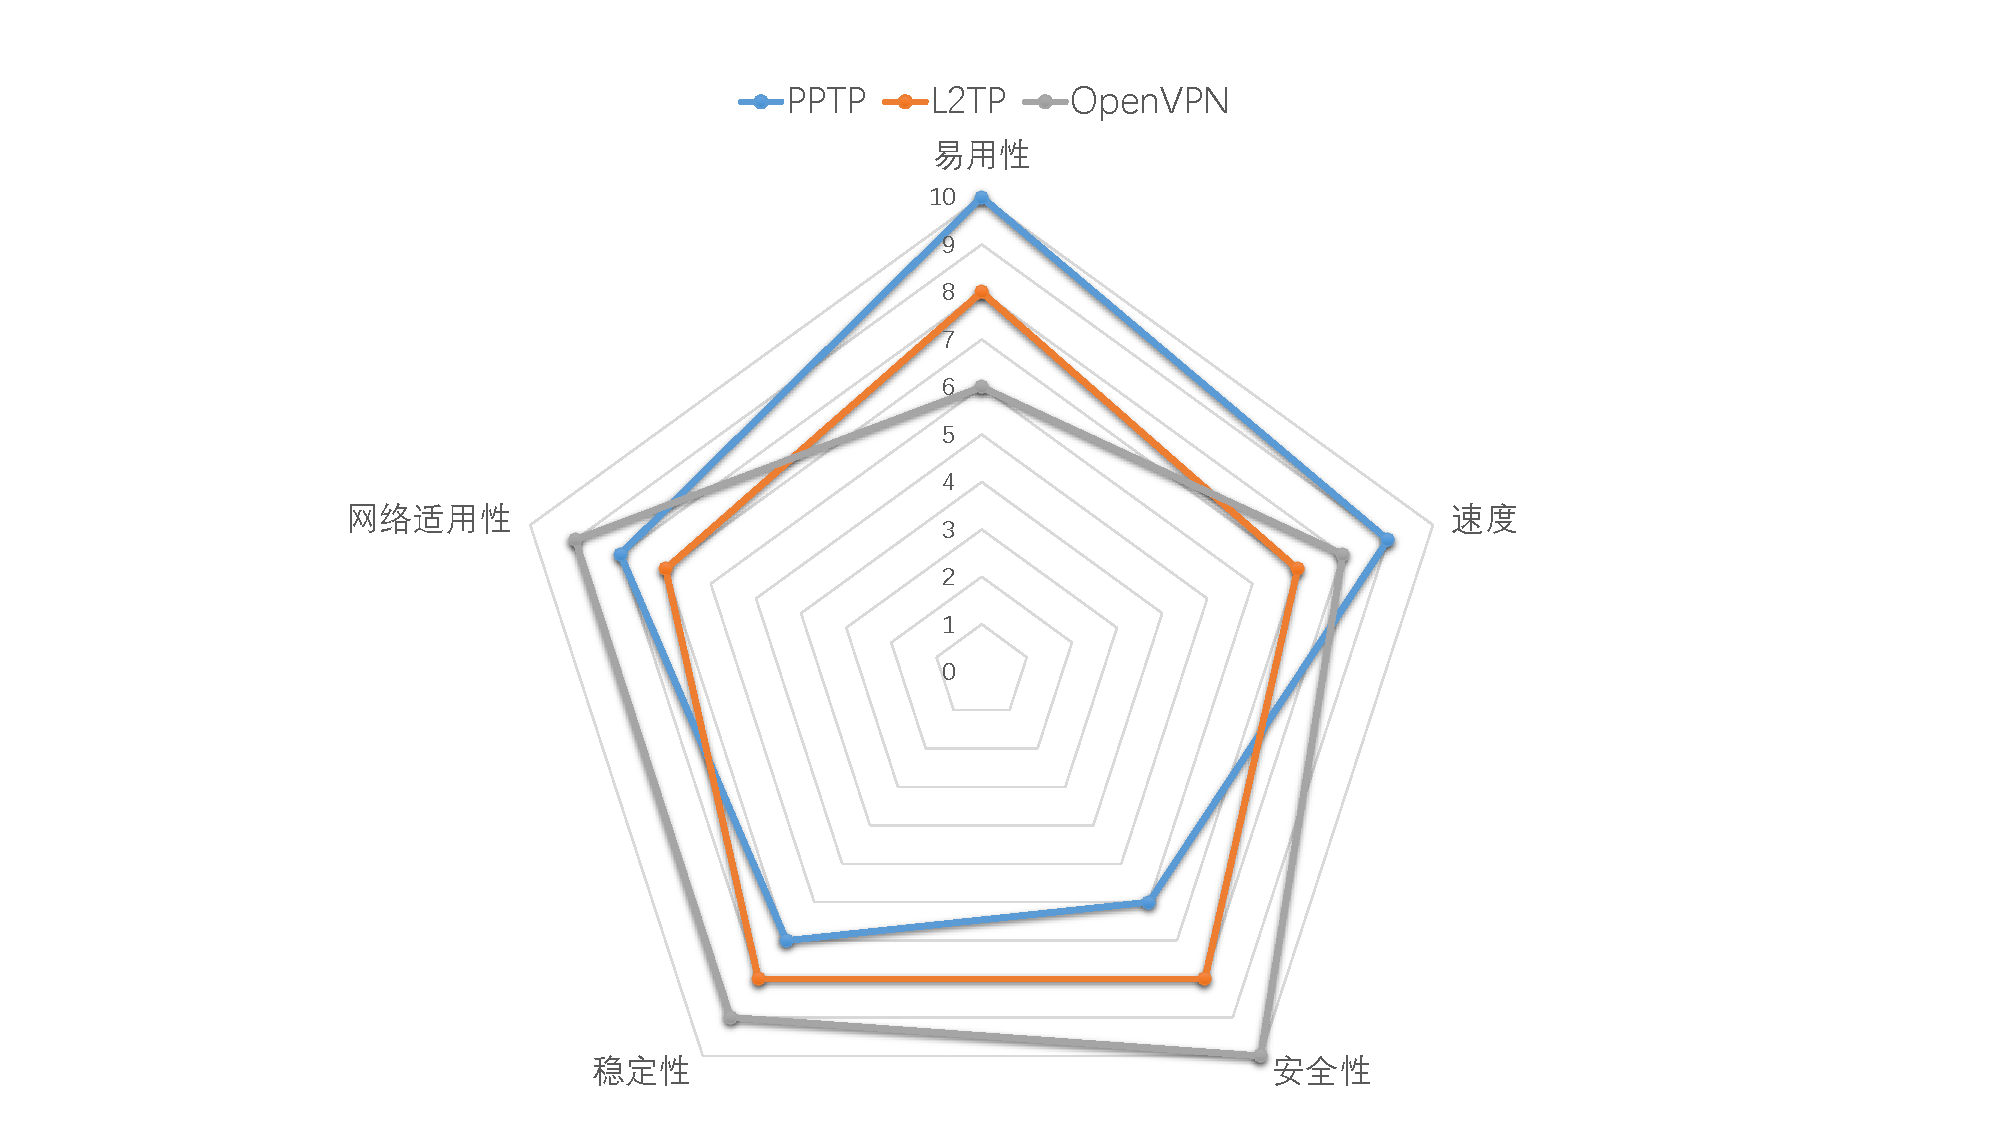
\includegraphics [width=1.0\textwidth]{figure//VPNCompare.pdf}
	\caption{VPN协议对比(1)}\label{VPNCompare}
\end{figure}

在图2.1中可以看到,PPTP协议在易用性和速度方面是有优势的,但是OpenVPN则在稳定性、安全性
和网络适用性上更胜一筹,而L2TP协议则是一种比较折中的方案。另外也找了网上的一些关于VPN的
对比,如图2.2所示:
\begin{figure}[hbtp]
	\centering
	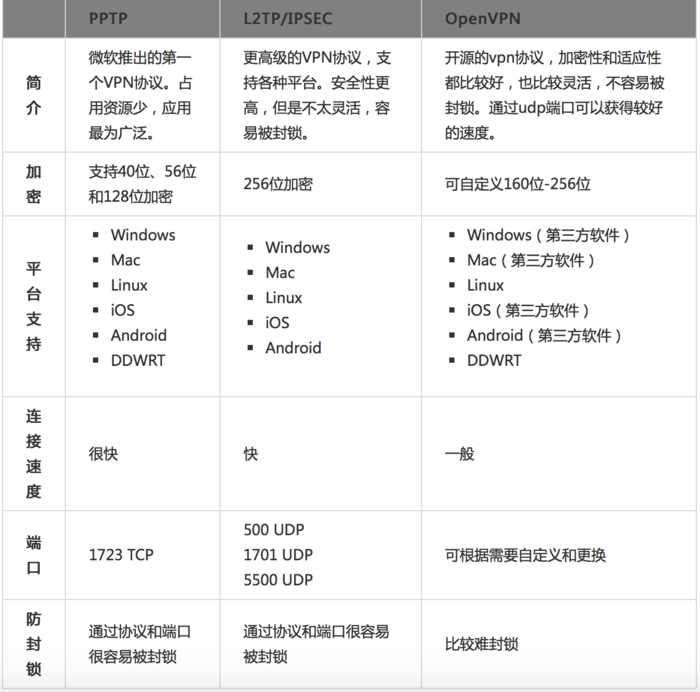
\includegraphics [width=0.5\textwidth]{figure//VPNCompare_01.png}
	\caption{VPN协议对比(2)}\label{VPNCompare_01}
\end{figure}

在雷达系统中稳定性和安全性是更应该被着重考虑的因素,综合来看在雷达系统网络管理中采用
OpenVPN方案是一种更加合适的选择。

\section{OpenVPN介绍}
VPN直译就是虚拟专用通道,是提供给企业之间或者个人与公司之间安全数据传输的隧道,OpenVPN
无疑是Linux下开源VPN的先锋,提供了良好的性能和友好的用户GUI。使用了OpenSSL加密库中的
SSLv3/TLSv1协议函数库,使得数据安全性更加的有保障。目前OpenVPN能在Solaris、Linux、
OpenBSD、FreeBSD、NetBSD、Mac OS X与Microsoft Windows以及Android和iOS上运行,并包
含了许多安全性的功能。

\begin{figure}[hbtp]
	\centering
	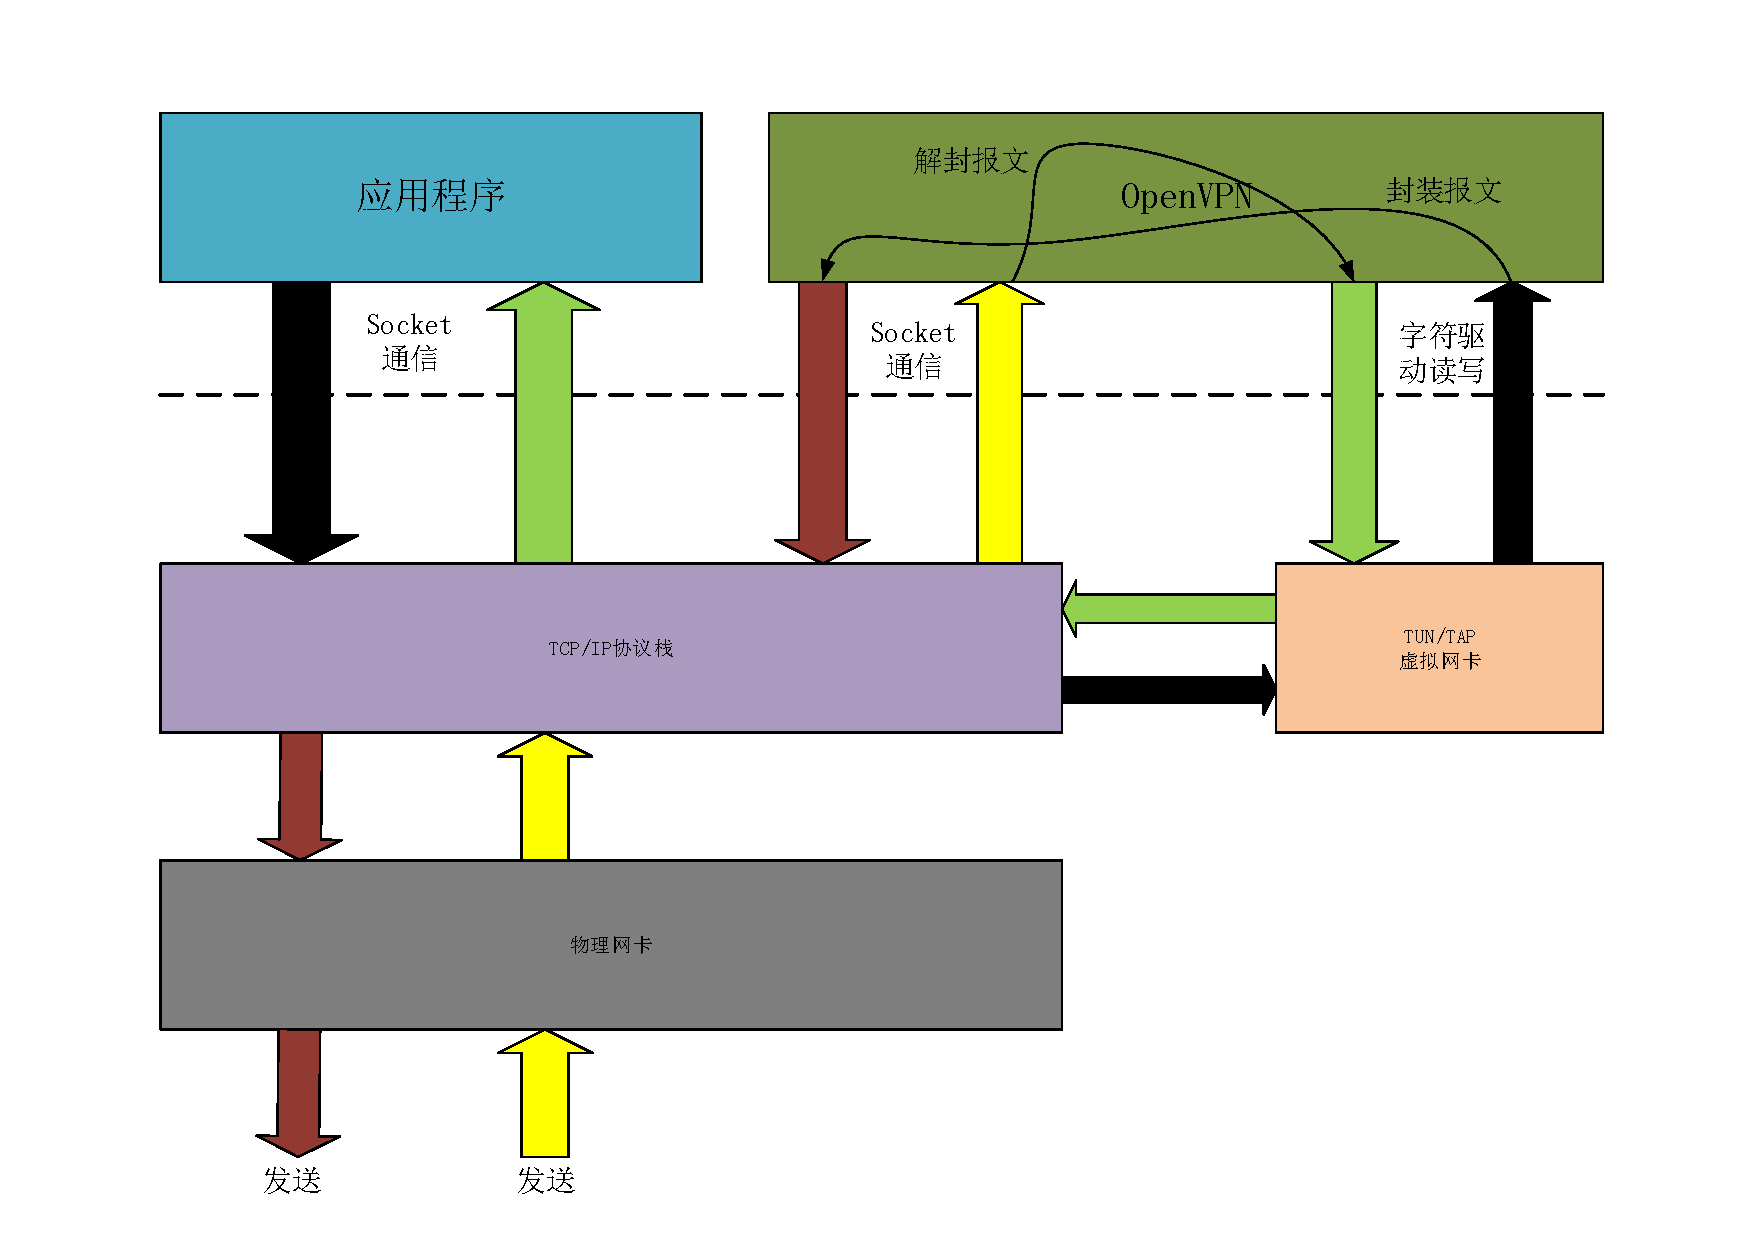
\includegraphics [width=0.6\textwidth]{figure//VPNPrince.pdf}
	\caption{OpenVPN原理}\label{VPNPrince}
\end{figure}

OpenVPN基本工作原理,如图2.3所示,应用层的外出数据,经过系统调用接口传入核心
TCP/IP层做处理,在TCP/IP经过路由到虚拟网卡,虚拟网卡的网卡驱动发送处理程序
hard\_start\_xmit()将数据包加入skb表并完成数据包从核心区到用户区的复制,OpenVPN调用虚
拟网卡的字符处理程序tun\_read(),读取到设备上的数据包,对读取的数据包使用SSL协议做封装
处理后,通过socket系统调用发送出去。 物理网卡接收数据包,经过核心TCP/IP上传到OpenVPN,
OpenVPN通过link\_socket\_read()接收数据包,使用SSL协议进行解包处理,经过处理的数据包
OpenVPN调用虚拟网卡的字符处理程序tun\_write()写入虚拟网卡的字符设备,设备驱动程序完成
数据从用户区到核心区的复制,并将数据写入skb链表,然后调用网卡netif\_rx()接收程序,数据
包再次进入系统TCP/IP协议栈,传到上层应用程序。如果想要了解更详细可以参考官方网站
\cite{OpenVPN.web}。


%---------------------------------------------------------------------
%  第三章
%---------------------------------------------------------------------
\chapter{网络安全}
网络的安全性是在部署远程控制网络时另外一个需要重点考虑的问题,本文提出可以从OpenVPN自身
安全策略和防火墙(Firewall)安全策略两方面来保障网络的安全性。
\section{OpenVPN安全策略}
OpenVPN提供的安全策略主要有以下几个方面:
\begin{itemize}
\itemsep=3pt
\parskip=0pt
\setlength{\itemindent}{1em} 
\item 认证证书机制,用户需要通过VPN服务器分发的认证证书才能接入服务端
\item 用户名和密码机制,每个客户端可以设置不同的用户名和密码 
\item 传输数据加密机制,保障所传输的数据是安全可靠的
\end{itemize}

可以看到OpenVPN提供了多重的网络和数据安全保障,在此基础上还需要配合防火墙策略来进行各个
区域的权限控制。

\section{Firewall策略}
根据雷达系统网络控制的需求,可以确定以下几点的防火墙策略原则:
\begin{itemize}
\itemsep=3pt
\parskip=0pt
\setlength{\itemindent}{1em} 
\item[-] 每个接入虚拟专网的区域均需要添加防火墙策略
\item[-] 权限区分,管理中心、研发中心和数据中心需要更高权限,雷达站则是低权限
\item[-] 设置管理员权限,可以访问网络上所有设备
\end{itemize}

根据确定的防火墙策略制定原则,可以制定雷达系统网络管理的一些基本防火墙策略,如表3.1所示,
由表可以看到管理员用户是可以访问所有网段的,主要用于维护整个网络和进行相关的配置,属于
admin权限,长沙研发中心用户和北京数据中心用户可以访问所有雷达站点设备和VPN服务器,属于
user权限,各个雷达站的则是connetor权限,只能访问VPN服务器。
\begin{table}[H]
	\centering
	\begin{tabular}{|l|c|c|c|}
	\hline
	类别            & IP地址           & 权限级别    & 备注\\
	\hline
	管理员          & 172.16.10.0/24   & admin      & 可以访问所有网段\\
	\hline
	长沙研发中心用户 & 172.16.11.0/24   & user       & 只能访问VPN服务器和雷达站网段\\
	\hline
	北京数据中心用户 & 172.16.12.0/24   & user       & 只能访问VPN服务器和雷达站网段\\
	\hline
	长沙雷达站设备   & 172.16.100.0/24  & connector  & 只能访问VPN服务器\\
	\hline
	佛山雷达站设备   & 172.16.101.0/24  & connector  & 只能访问VPN服务器\\
	\hline
	上海雷达站设备   & 172.16.102.0/24  & connector  & 只能访问VPN服务器\\
	\hline
	...    		& ...             & ... & ...\\
	\hline
	\end{tabular}
	\caption{Firewall策略}
	\label{tab:FirewallPolicy }
\end{table}

如果使用图来表示将会更加清晰,在图3.1中,红色区域表示admin区域,绿色区域表示user区域,
黄色区域表示connector区域。

\begin{figure}[hbtp]
	\centering
	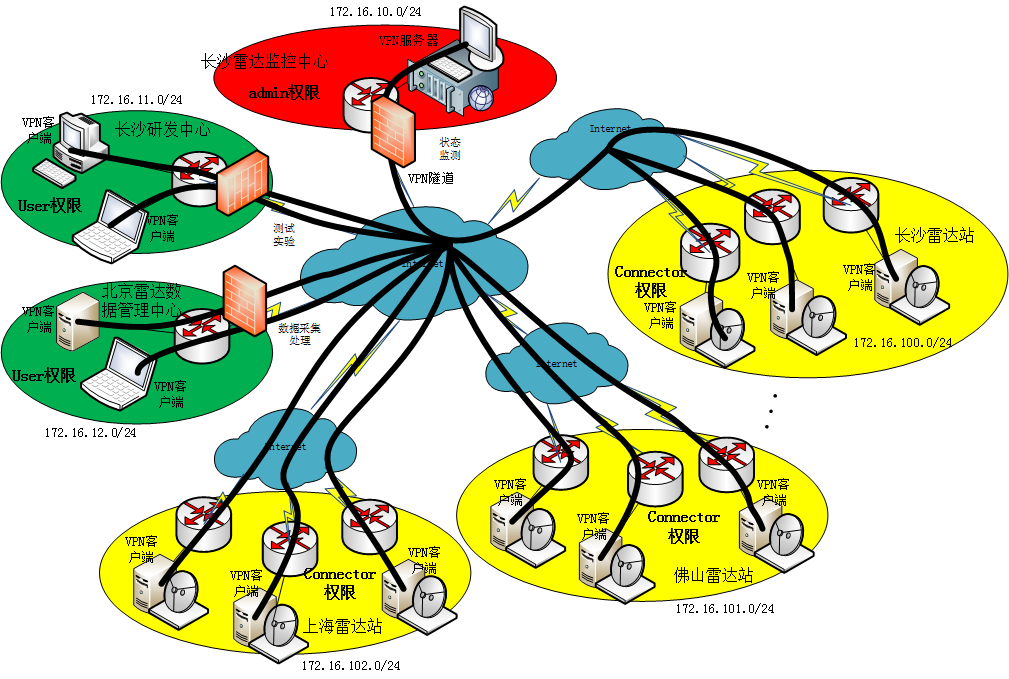
\includegraphics [width=1.0\textwidth]{figure//RadarPrivilege.png}
	\caption{防火墙策略区域}\label{RadarPrivilege}
\end{figure}
%---------------------------------------------------------------------
%  第四章
%---------------------------------------------------------------------
\chapter{配置步骤}

\begin{spacing}{1.5}
\section{OpenVPN安装}
OpenVPN官方基本提供了多个平台的OpenVPN包,在Windows平台可以直接安装Openvpn安装包,本
节主要介绍在Linux平台编译安装OpenVPN包。在编译OpenVPN软件前最好先编译安装openssl软件,
因为OpenVPN调用了Openssl函数库,OpenVPN的客户端和服务端建立SSL链接的过程是通过调用
Openssl来实现的。

在下载好的源码包中,有个INSTALL文件,里面有具体的安装步骤和注意事项,可按需进行查阅。
进入openvpn目录,需要手动生成编译脚本configure。

\begin{tcolorbox}[notitle,boxrule=0pt,colback=gray!20,colframe=gray!20]
autoreconf -i -v -f 
{\color{red} 
//BUILD COMMANDS FROM SRC REPOSITORY CHECKOUT
}
\end{tcolorbox}

生成configure脚本之后就可以执行configure脚本了:
\begin{tcolorbox}[notitle,boxrule=0pt,colback=gray!20,colframe=gray!20]
./configure --prefix=/usr/local/OpenVPN --disable-lzo  
{\color{red} 
//如需禁用lzo,加入此参数
}

make

make install
\end{tcolorbox}
编译完成之后默认是安装在/usr/local目录下的,如果需要改变安装目录,在./configure时添加
--prefix=PREFIX即可,或者直接建立软连接。
\begin{tcolorbox}[notitle,boxrule=0pt,colback=gray!20,colframe=gray!20]
ln -s /usr/local/OpenVPN/sbin/openvpn /usr/sbin/openvpn
\end{tcolorbox}

\section{OpenVPN配置}
OpenVPN的配置是分成几个阶段的,第一阶段先需要进行密钥的生成,第二阶段才是具体的OpenVPN
功能的配置,下面分成两个小节来叙述OpenVPN配置。

\subsection{密钥配置}
要完成OpenVPN的密钥配置需要先安装配置easy-rsa,且基于easy-rsa3来进行配置。easy-rsa源
文件需要从github进行下载\cite{easy-rsa.web},其和OpenVPN是在同一个软件库。完成下载之
后按照下面的步骤进行配置。
\begin{tcolorbox}[notitle,boxrule=0pt,colback=gray!20,colframe=gray!20]
mkdir /etc/openvpn

mkdir /usr/local/OpenVPN/etc

ln -s /usr/local/OpenVPN/etc /etc/openvpn

cd easyrsa3/

cp vars.example vars
\end{tcolorbox}
主要需要对vars中的一些选项进行配置,具体修改如图4.1,
\begin{figure}[hbtp]
	\centering
	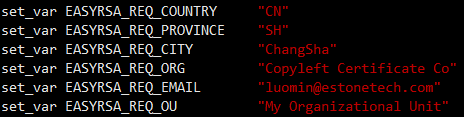
\includegraphics [width=0.8\textwidth]{figure//vars_01.png}
	\caption{vars文件修改}\label{vars_01}
\end{figure}

接下来,开始初始化pki:
\begin{tcolorbox}[notitle,boxrule=0pt,colback=gray!20,colframe=gray!20]
./easyrsa init-pki
\end{tcolorbox}

创建根证书CA:
\begin{figure}[hbtp]
	\centering
	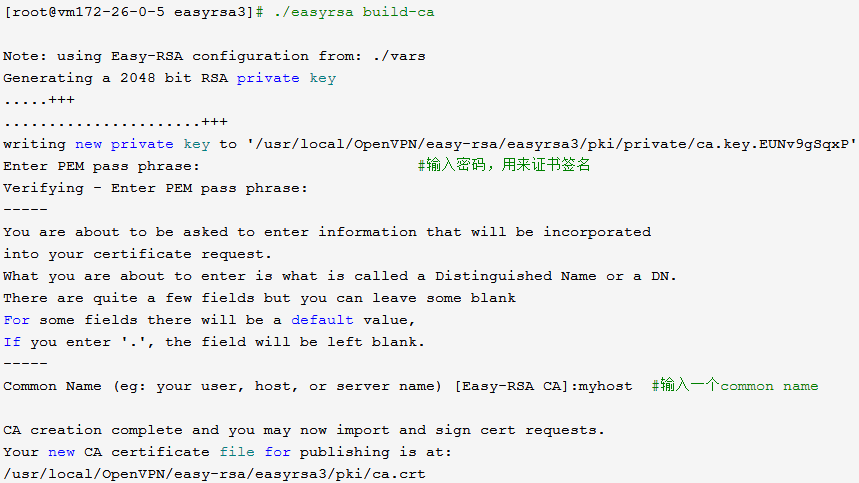
\includegraphics [width=0.8\textwidth]{figure//build-ca.png}
	\caption{创建根证书}\label{build-ca}
\end{figure}

创建服务器端证书:
\begin{figure}[hbtp]
	\centering
	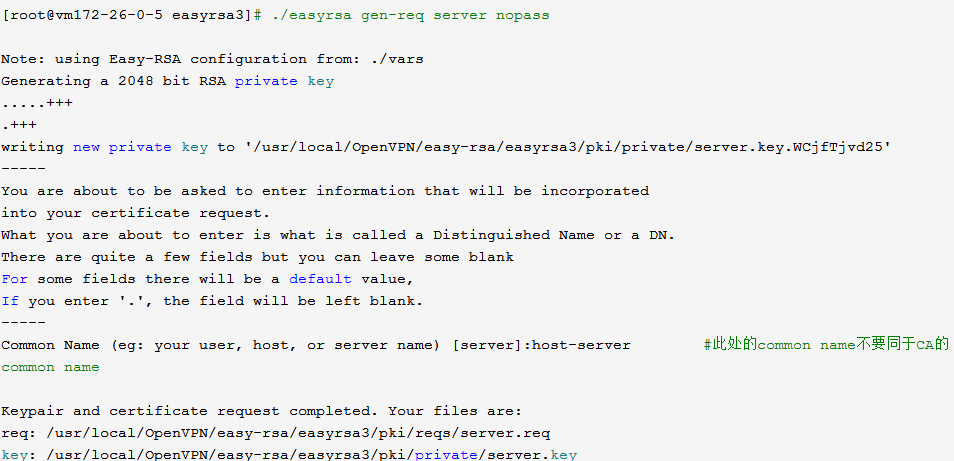
\includegraphics [width=0.8\textwidth]{figure//server-ca.png}
	\caption{创建服务器端证书}\label{server-ca}
\end{figure}


签约服务器端证书:
\begin{figure}[H]
	\centering
	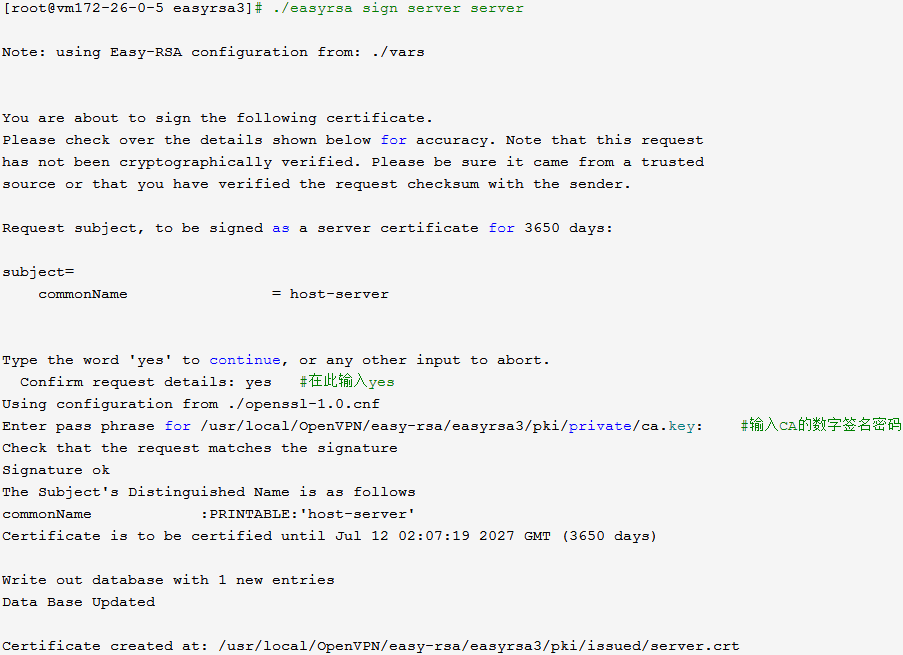
\includegraphics [width=0.8\textwidth]{figure//sign-server-ca.png}
	\caption{签约服务器端证书}\label{sign-server-ca}
\end{figure}

创建Diffie-Hellman,确保key穿越不安全网络:
\begin{figure}[H]
	\centering
	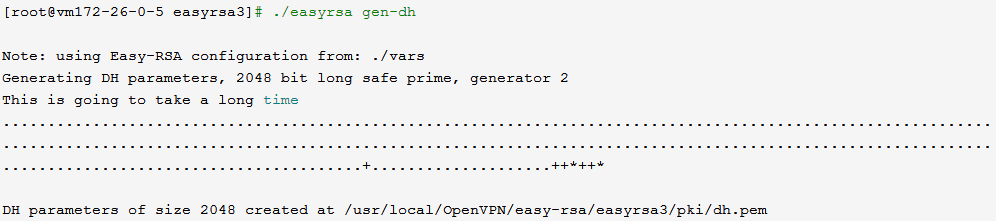
\includegraphics [width=0.8\textwidth]{figure//gen-dh.png}
	\caption{创建Diffie-Hellman}\label{gen-dh}
\end{figure}

同样的在客户端也是需要证书的,需要在另外一个路径clone一份easyrsa源码。然后进入源码执行
初始化操作。
\begin{tcolorbox}[notitle,boxrule=0pt,colback=gray!20,colframe=gray!20]
./easyrsa init-pki
\end{tcolorbox}

生成客户端证书生成请求和key:
\begin{figure}[hbtp]
	\centering
	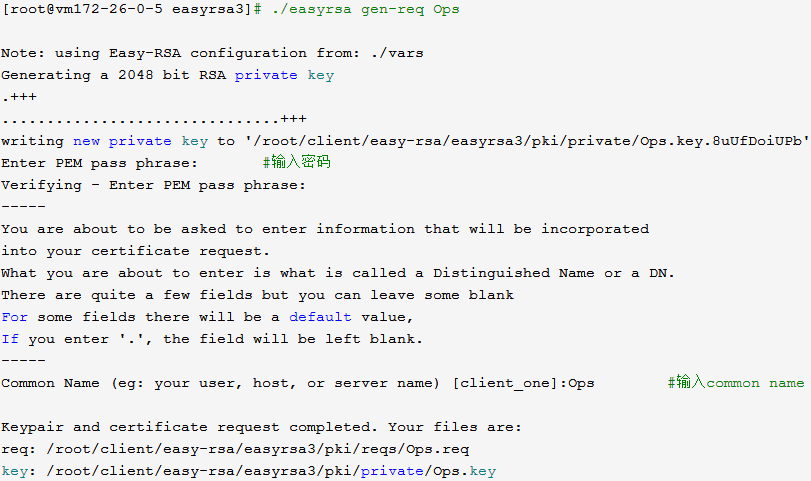
\includegraphics [width=0.8\textwidth]{figure//client-ca.png}
	\caption{创建客户端证书}\label{client-ca}
\end{figure}

执行下面的命令导入客户端证书:

\begin{tcolorbox}[notitle,boxrule=0pt,colback=gray!20,colframe=gray!20]
cd /usr/local/OpenVPN/easy-rsa/easyrsa3

./easyrsa import-req  /root/client/easy-rsa/easyrsa3/pki/reqs/Ops.req Ops
\end{tcolorbox}

签约客户端证书:
\begin{figure}[H]
	\centering
	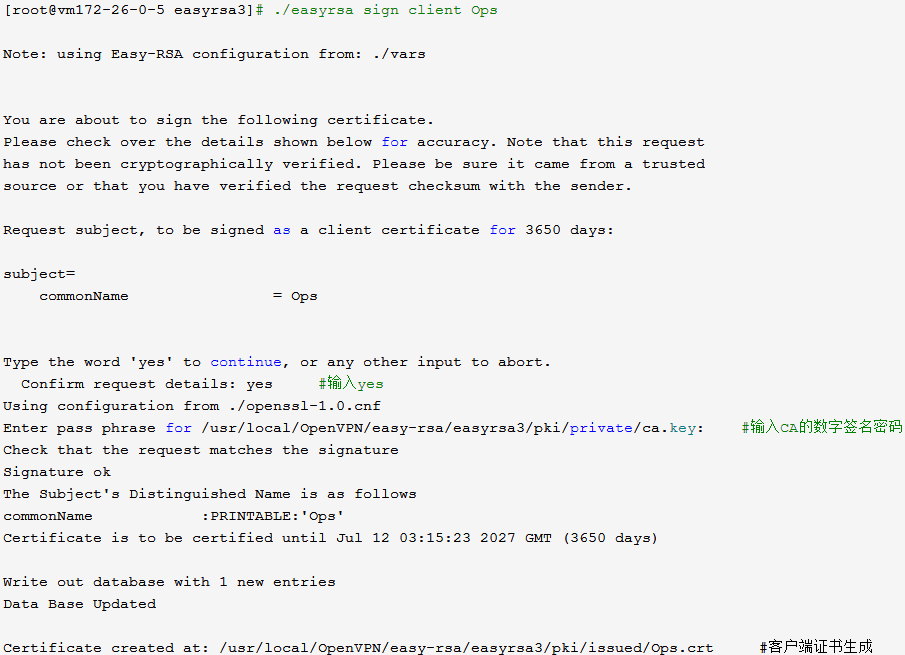
\includegraphics [width=0.8\textwidth]{figure//sign-client-ca.png}
	\caption{签约客户端证书}\label{sign-client-ca}
\end{figure}

至此,客户端和服务端的证书已经配置完毕,接下来将相关文件拷贝至openvpn安装目录下:

\begin{tcolorbox}[notitle,boxrule=0pt,colback=gray!20,colframe=gray!20]
cp ca.crt /etc/OpenVPN/

cp private/server.key /etc/Openvpn/

cp issued/server.crt /etc/Openvpn/

cp dh.pem /etc/Openvpn/
\end{tcolorbox}

拷贝客户端证书和秘钥至客户端client目录,在后面客户机连接服务器的时候是会要用到的:

\begin{tcolorbox}[notitle,boxrule=0pt,colback=gray!20,colframe=gray!20]
cp ca.crt /root/client/

cp issued/Ops.crt /root/client/

cp /root/client/easy-rsa/easyrsa3/pki/private/Ops.key /root/client/
\end{tcolorbox}

本小节主要介绍了OpenVPN的密钥生成和配对,整个过程稍显复杂,不过OpenVPN的安全性便是由密
钥和证书来保证,所以这是必不可少的一个环节。

\subsection{网络配置}
本节主要介绍OpenVPN的一些基本网络配置,如下所示,列出了服务端server.conf文件的一些基本
配置,可以看到端口被配置成了2194,使用的通行模式是upd,配置的OpenVPN服务器网段为
172.16.10.0/24,相应的还配置了之前生成的密钥文件。

\begin{tcolorbox}[notitle,boxrule=0pt,colback=gray!20,colframe=gray!20]
port 5094

proto udp

dev tun

ca /etc/openvpn/ca.crt

cert /etc/openvpn/server.crt

key /etc/openvpn/server.key  \#This file should be kept secret

dh /etc/openvpn/dh.pem

server 172.16.10.0 255.255.255.0

ifconfig-pool-persist ipp.txt

keepalive 10 120

tls-auth /etc/openvpn/ta.key 0 \# This file is secret

cipher AES-256-CBC

persist-key

persist-tun

status /tmp/openvpn-status.log

verb 3

explicit-exit-notify 1
\end{tcolorbox}

可以再看一下客户端的配置文件client.conf,如下所示,主要配置了程序为client模式,设置了
服务器的地址及端口,以及上一节中介绍的相关客户端的证书和密钥。

\begin{tcolorbox}[notitle,boxrule=0pt,colback=gray!20,colframe=gray!20]
client

dev tun

proto udp

remote 218.76.8.148 5094

resolv-retry infinite

nobind

persist-key

persist-tun

ca /etc/openvpn/ca.crt

cert /etc/openvpn/Ops.crt

key /etc/openvpn/Ops.key

remote-cert-tls server

tls-auth /etc/openvpn/ta.key 1

cipher AES-256-CBC

verb 3

\end{tcolorbox}


\end{spacing}

%---------------------------------------------------------------------
%  第五章 总结 
%---------------------------------------------------------------------
\titleformat{\chapter}{\centering\zihao{-1}\heiti}{第\chinese{chapter}章}{1em}{}
\chapter{总结}
\begin{spacing}{1.5}
整个雷达系统的网络管理纷繁复杂,主要是因为设备和用户较多,并且需要各种不一样的权限划分,
数据需要远程传输,设备需要远程管理,各种安全性的要求也一一呈现。本文主要提出了采用
OpenVPN+Firewall的管理方案,在OpenVPN的基础上添加相关的防火墙策略,划分各个区域,确定
每个接入设备的IP地址和接入用户的使用权限。在相关配置都论述清楚的情况下,针对雷达系统的管
理也就变得清晰明了。
\end{spacing}

%---------------------------------------------------------------------
%  参考文献设置
%---------------------------------------------------------------------
\addcontentsline{toc}{chapter}{参考文献}

\begin{thebibliography}{99}
\songti \zihao{-4} 	
	\bibitem{OpenVPN.web}
	https://www.openvpn.net/
	\bibitem{easy-rsa.web}
	https://github.com/OpenVPN/easy-rsa.git
	
\end{thebibliography}

		
\end{document}